\newcommand{\scenario}[8]{
\begin{table}
    \centering
    \begin{tabular}{|l|}
        \hline
        \textbf{Identifikator}: #1\\
        \hline
        \textbf{Naziv}: #2\\
        \hline
        \textbf{Učesnik}: #3\\
        \hline
        \textbf{Opis}: #4\\
        \hline
        \textbf{Preduslovi}: #5\\
        \hline
        \textbf{Posledice}: #6\\
        \hline
        \textbf{Osnovni tok izvršavanja}\\
        \begin{minipage}{0.9\textwidth}
            \vskip 4pt
            \begin{enumerate}
                #7
            \end{enumerate}
            \vskip 4pt
        \end{minipage}\\
        \hline
        #8
    \end{tabular}
    \caption{#2}
\end{table}
}

\newcommand{\altflow}[2]{
    \textbf{Alternativni tok #1}\\
    \begin{minipage}{0.9\textwidth}
        \vskip 4pt
        \begin{enumerate}
            #2
        \end{enumerate}
        \vskip 4pt
    \end{minipage}\\
    \hline
}

\rhead{Dijagram slučajeva korišćenja}
\section{Dijagram slučajeva korišćenja}
U nastavku se nalazi dijagram slučajeva korišćenja [Slika \ref{fig:use-case}] na kome su prikazane pravila poslovanja.
\begin{figure}[h]
    \centering
    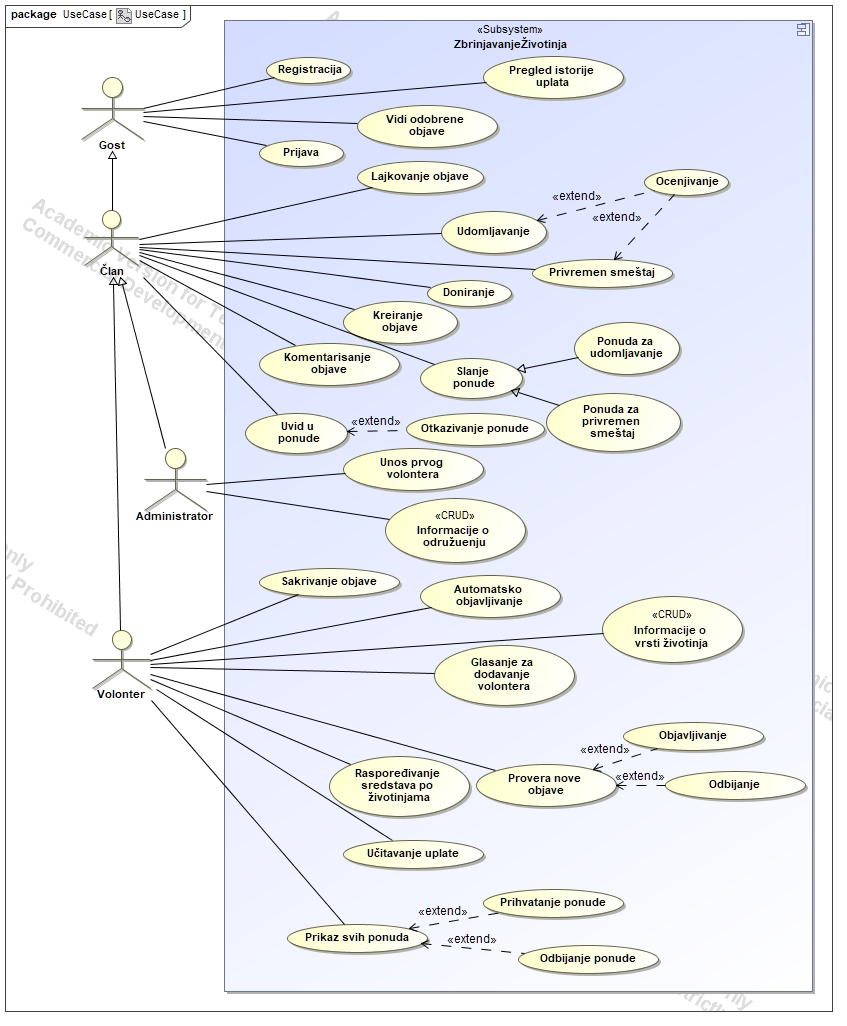
\includegraphics[width=\textwidth]{img/use-case.jpg}
    \caption{Dijagram slučajeva korišćenja}
    \label{fig:use-case}
\end{figure}
\subsection{Scenariji slučajeva korišćenja}
\par U nastavku se nalaze scenariji korišćenja prikazani na dijagramu slučajeva korišćenja [Slika \ref{fig:use-case}].
\scenario{GI1}
        {Registracija}
        {Gost}
        {Gost se registruje na sistem}
        {Otvorena registraciona forma}
        {Gost ima mogućnost da se prijavi na sistem}
        {
            \item Gost unosi ime, prezime, adresu, datum rođenja, pol i broj telefona.
            \item Sistem proverava validnost podataka.
            \item Sistem obaveštava gosta da je registracija prošla uspešno. [Alternativni tok A]
            \item Kraj scenarija.
        }
        {
            \altflow{A: Neispravno uneti podaci}
            {
                \item Sistem obaveštava gosta o greškama u formi.
                \item Prikazuje se forma za registraciju.
                \item Kraj scenarija.
            }
        }
\scenario{GI2}
          {Vidi odobrene objave}
          {Gost}
          {Prikaz odobrenih objava gostu}
          {Nema preduslova}
          {Član može da vidi odobrene objave}
          {
            \item Sistem učitava sve odobrene objave.
            \item Kraj scenarija.
          }
          {}

\scenario{GI3}
         {Pregled istorije uplata}
         {Gost}
         {Prikaz svih prethodnih donacija}
         {Pritisnuto je dugme za prikaz istoje donacija}
         {član može da vidi sve prethodne donacije}
         {
            \item Sistem učitava istoriju donacija.
            \item Kraj scenarija
         }
         {}


\scenario{GI4}
        {Prijava}
        {Gost}
        {Prijava člana na sistem unosom korisničkog imena i šifre}
        {Otvorena je forma za prijavu}
        {član može da koristi funkcionalnosti sistema}
        {
            \item Član unosi korisničko ime i šifru.
            \item Sistem proverava da li su korisničko ime i šifra ispravni.
            \item Sistem otvara odgovarajući meni [Alternativni tok A]
            \item Kraj scenarija.
        }
        {
            \altflow{A: Neispravno korisničko ime ili šifra}
            {
                \item Sistem obaveštava člana da su korisničko ime ili šifra neispravni.
                \item član potvrđuje da je video obaveštenje.
                \item Prikazuje se forma za prijavu.
                \item Kraj scenarija.
            }
        }

\scenario{GI5}
         {Doniranje}
         {Član}
         {Prikaz informacija za donacije}
         {\makecell[l]{član je prijavljen na sistem i dugme za donacije \\je pritisnuto}}
         {A: Član ima informacije potrebne za slanje donacije}
         {
            \item Sistem prikazuje informacije o bankovnom računu
            \item Kraj scenarija
         }
         {}

\scenario{MI1}
         {Zahtev za promociju u volontera}
         {Član}
         {Član šalje zahtev za promociju u volontera}
         {Član je prijavljen na sitem}
         {Zahtev je zabeležen u sistemu}
         {
            \item Član unosi razlog za promociju.
            \item Sistem obaveštava člana da je zahtev uspešno poslat.
            \item Sistem trajno čuva zahtev.
            \item Kraj scenarija.
         }{}

\scenario{MI2}
         {Označava objavu da mu se sviđa}
         {Član}
         {Član označava objavu da mu se sviđa}
         {Član je prijavljen na sistem}
         {Promenjen broj sviđanja na objavi}
         {
            \item Sistem vizuelno obaveštava da mu se objava sviđa.
            \item Sistem dodaje člana u listu sviđanja za objavu.[Alternativni tok A]
            \item Kraj scenarija.
         }
         {
            \altflow{A: Član je već označio da mu se objava sviđa}
            {
                \item Sistem uklanja člana iz liste sviđanja za objavu.
                \item Kraj scenarija.
            }
         }

\scenario{MI3}
         {Komentarisanje objave}
         {Član}
         {Član komentariše objavu}
         {Član je prijavljen na sistem}
         {Dodat novi komentar na objavu}
         {
            \item Član unosi komentar.
            \item Sistem dodaje komentar na objavu.
            \item Kraj scenarija.
         }
         {}

\scenario{MI4}
         {Uvid u ponude}
         {Član}
         {Član ima uvid u sve njehgve ponude. EP1 Član otkazuje ponudu}
         {\makecell[l]{Član je prijavljen na sistem. Pritisnuto je dugme\\ za prikaz ponuda}}
         {Nema posledica.}
         {
            \item Sistem prikazuje sve njegove ponude.
            \item $[$Tačka proširenja: EP1 Otkazivanje ponude$]$
            \item Kraj scenarija.
         }
         {}

\scenario{EP1}
        {Otkazivanje ponude}
        {Član}
        {Otkazivanje članove ponude}
        {Otvoren je prikaz članovih ponuda.}
        {Članova odluka se trajno čuva.}
        {
            \item Član aktivira brisanje ponude.
            \item Sistem obaveštava člana o posledicama otkazivanja.
            \item Član pritiska dugme otkaži. [Alternativni tok A]
            \item Sistem briše ponudu iz sistema i osvežava meni sa ponudama.
            \item Kraj scenarija.
        }
        {
            \altflow{A: Član odustaje od brisanja}
            {
                \item Sistem osvežava meni sa ponudama.
                \item Kraj scenarija.
            }
        }